\documentclass[12pt,a4paper]{article}

% --------------------------------------------------
% Encoding and Fonts
% --------------------------------------------------
\usepackage[T1]{fontenc}
\usepackage[utf8]{inputenc}
%\usepackage{lmodern}

% --------------------------------------------------
% Page Layout
% --------------------------------------------------
\usepackage{geometry}
\geometry{margin=1.2in}

% --------------------------------------------------
% Microtypography
% --------------------------------------------------
%\usepackage{microtype}

% --------------------------------------------------
% Mathematics
% --------------------------------------------------
\usepackage{amsmath,amssymb,amsthm,mathtools}

% --------------------------------------------------
% Figures and Tables
% --------------------------------------------------
\usepackage{graphicx}
\usepackage{booktabs}
\usepackage{tikz}
\usetikzlibrary{arrows.meta, positioning, calc, decorations.pathmorphing}

% --------------------------------------------------
% Citations
% --------------------------------------------------
\usepackage{natbib}

% --------------------------------------------------
% Hyperlinks
% --------------------------------------------------
\usepackage{hyperref}
\hypersetup{
  colorlinks=true,
  linkcolor=black,
  citecolor=black,
  urlcolor=blue
}

% --------------------------------------------------
% Spacing and Layout Utilities
% --------------------------------------------------
\usepackage{setspace}
\setstretch{1.15}
\usepackage{enumitem}

% --------------------------------------------------
% Theorem Environments
% --------------------------------------------------
\theoremstyle{definition}
\newtheorem{definition}{Definition}[section]

\theoremstyle{plain}
\newtheorem{theorem}[definition]{Theorem}
\newtheorem{proposition}[definition]{Proposition}
\newtheorem{lemma}[definition]{Lemma}
\newtheorem{corollary}[definition]{Corollary}

\theoremstyle{remark}
\newtheorem{remark}[definition]{Remark}
\newtheorem{example}[definition]{Example}

% --------------------------------------------------
% Custom Macros
% --------------------------------------------------
\newcommand{\HX}{H(X)}
\newcommand{\HY}{H(Y)}
\newcommand{\HE}{H_{E}}
\newcommand{\calL}{\mathcal{L}}
\newcommand{\calS}{\mathcal{S}}
\newcommand{\calC}{\mathcal{C}}
\newcommand{\calG}{\mathcal{G}}
\newcommand{\calX}{\mathcal{X}}
\newcommand{\calY}{\mathcal{Y}}
\newcommand{\Prob}{\mathbb{P}}

% --------------------------------------------------
% Title Information
% --------------------------------------------------
\title{Normalization Without Convergence:\\[6pt]
Large Language Models, Linguistic Entropy,\\
and the Myth of Cognitive Homogenization}

\author{Flyxion}

\date{}

% --------------------------------------------------
% Document
% --------------------------------------------------
\begin{document}

\maketitle

\begin{abstract}
Recent commentary in cognitive science and computational linguistics has proposed that large
language models (LLMs) are driving a broad homogenization of human language, perspective, and
reasoning. According to this view, the widespread use of generative systems encourages
convergence toward a statistical ``median'' embedded in the models' training distributions,
potentially narrowing the diversity of linguistic expression and epistemic viewpoints across
communicating populations. While this hypothesis raises important questions about the
long-run cultural consequences of AI-mediated communication, many existing formulations rest
on an implicit and underexamined assumption: that linguistic output provides a transparent
window into the underlying generative structure of human cognition.

This paper argues that such claims systematically conflate two distinct phenomena:
\emph{surface-level normalization in the communication channel} and \emph{deep convergence in
the generative processes of human cognition}. Drawing on an information-theoretic framework,
we demonstrate that a system capable of mapping many idiosyncratic inputs to a standardized
representation necessarily reduces the entropy of observable outputs while leaving the entropy
of the underlying source distribution unchanged or unaffected. Formally, this follows from
the data-processing inequality: post-processing cannot increase mutual information. In other
words, uniformity at the level of representational output does not entail---and cannot
establish---homogenization at the level of thought.

From this perspective, large language models function less as normative enforcement mechanisms
than as \emph{translation layers} between heterogeneous private linguistic systems and shared
public registers. By reducing the communicative cost of nonstandard spelling, dialect, or
multilingual composition, such systems may in fact expand the effective expressive space
available to individual authors. We formalize this argument through a source--channel model,
develop the notion of \emph{linguistic attractor basins} in a probabilistic landscape, and
introduce a distinction between the entropy of generative sources and the entropy of
exploratory discovery processes.

We further argue that the more significant ecological risk of LLM-mediated communication lies
not in stylistic convergence but in the potential contraction of \emph{exploratory variance}
in knowledge discovery: the diversity of trajectories through which individuals encounter
novel ideas, conflicting interpretations, and unexpected conceptual recombinations. If
model-mediated search increasingly directs users toward the same conceptual summaries and
canonical explanations, the space of intellectual trajectories may contract even while
expressive diversity at the surface level remains intact. Understanding the cultural
consequences of generative AI therefore requires attention not only to the entropy of
linguistic form but also to the information ecology of exploration, discovery, and conceptual
variation.
\end{abstract}

\newpage
\tableofcontents
\newpage

% ==================================================
\section{Introduction}
\label{sec:introduction}
% ==================================================

Technologies that mediate human communication have repeatedly and profoundly reshaped the
structure of linguistic expression and intellectual exchange. Writing systems, printing
presses, editorial institutions, telegraph networks, search engines, and digital archives have
each altered the mechanisms through which language is produced, transmitted, and interpreted.
These transformations have recurrently generated concerns about the potential homogenization
of thought: that the machinery of communication will ultimately flatten the diversity of the
minds it connects. Yet the historical record consistently resists this conclusion. The
diffusion of moveable type standardized orthographic conventions across European languages
without destroying the intellectual heterogeneity of the Reformation. Editorial institutions
imposed consistent rhetorical styles on scientific writing without constraining the diversity
of scientific ideas. The internet concentrated written discourse around a small number of
dominant platforms without eliminating the extraordinary proliferation of viewpoints that
those platforms carry. In each case, normalization in the communication channel coexisted with
the persistence or even expansion of cognitive diversity at the level of the source.

The emergence of large language models (LLMs) represents the latest development in this long
sequence of communicative technologies. Generative AI systems are now widely used to assist
with writing, translation, summarization, coding, and information retrieval. Because these
systems produce text by sampling from probability distributions learned from large corpora,
their outputs often reflect statistically common linguistic forms: frequently recurring
syntactic constructions, standard rhetorical organization, and stylistically moderate
registers. This characteristic has prompted a growing body of scholarly commentary suggesting
that the widespread adoption of LLMs may gradually homogenize human language, perspective,
and reasoning---that individual discourse will be pulled, through repeated interaction with
shared systems, toward a common statistical center.

The homogenization hypothesis raises important questions regarding the long-term cultural
consequences of AI-mediated communication. If a large and growing proportion of human
discourse becomes filtered through a small set of generative systems, the observable
distribution of linguistic expression may indeed shift toward a common mode. Such a shift
could plausibly influence not only the stylistic surface of language but the structure of
argumentation and the framing of ideas. These are legitimate concerns that deserve serious
analytical treatment.

However, evaluating the homogenization hypothesis requires careful attention to a distinction
that much of the existing literature has failed to draw clearly: the distinction between
\emph{observable representations} and the \emph{generative processes} that produce them.
Communication systems routinely include intermediate transformation layers that reshape
linguistic signals during transmission without altering the cognitive diversity of the
communicating agents. Spelling conventions normalize orthographic variation. Editorial
practices standardize rhetorical structure. Translation systems project expressions across
language boundaries. Each of these mechanisms compresses surface-level variation without
penetrating the generative layer of cognition.

Large language models can be interpreted as a technologically novel form of such
normalization. When used as editing or translation tools, they map diverse linguistic inputs
into standardized outputs. The resulting reduction in observable variability may therefore
reflect the operation of the communication channel rather than any transformation of the
generative source. If this interpretation is correct, the inference from observed output
uniformity to cognitive convergence is formally invalid.

This paper develops a theoretical framework for analyzing this distinction with precision,
drawing on concepts from information theory, probabilistic modeling, and the ecology of
knowledge systems. The central claim is that the homogenization thesis systematically conflates
two distinct kinds of entropy reduction: compression within the communication channel, which
is a property of the transformation, and convergence within the generative processes of human
cognition, which is a claim about the source distribution.

The analysis is organized as follows. Section~\ref{sec:homogenization} introduces the
homogenization hypothesis in its principal variants and identifies the shared inferential
assumptions that underlie them. Section~\ref{sec:sourceentropy} develops an
information-theoretic framework distinguishing source entropy from channel entropy and
establishes the central formal results. Section~\ref{sec:private} elaborates the distinction
between private generative systems and public communicative registers, drawing on historical
precedent. Section~\ref{sec:instrumental} analyzes the difference between instrumental and
epistemic uses of generative models and their differential implications for cognitive
influence. Sections~\ref{sec:attractor}--\ref{sec:landscape} develop the geometric notion
of linguistic attractor basins and the conceptual landscape in which they reside.
Section~\ref{sec:exploratory} introduces the concept of exploratory entropy and analyzes
how algorithmic mediation reshapes discovery distributions. Sections~\ref{sec:sourati}
and~\ref{sec:agenda} engage with the specific claims of recent empirical literature and
propose a more precise research program. Section~\ref{sec:prostheses} situates LLMs within
a broader history of cognitive prosthetic technologies. Section~\ref{sec:conclusion} draws
the threads together and states the paper's principal conclusions. Appendices provide more
detailed derivations of the central entropy results and a formal treatment of rank-mediated
discovery distributions.

% ==================================================
\section{The Homogenization Thesis}
\label{sec:homogenization}
% ==================================================

Recent discussions in cognitive science and computational linguistics have articulated a
growing concern that large language models may induce a progressive homogenization of human
language, reasoning, and perspective. The core intuition motivating this family of claims is
straightforward. Because LLMs are trained on large corpora that aggregate statistical
regularities across vast quantities of human communication, their outputs tend to reflect the
most probable linguistic forms and conceptual framings present in those datasets. When such
systems are widely adopted as writing assistants, editors, and conversational partners, it is
argued that human discourse may gradually converge toward the same statistical center that
those systems implicitly represent \citep{sourati2026}.

In this view, the widespread use of generative language models acts as a powerful attractor
within the space of linguistic and epistemic practices. Individual expressions that initially
vary across dialects, registers, educational backgrounds, and cultural contexts are
progressively ``pulled'' toward a shared normative distribution. Over time, this process is
thought to reduce variance across several dimensions of human communication simultaneously:
lexical choice, rhetorical structure, argumentative form, and epistemic framing.

The homogenization thesis appears in three structurally distinct but related variants that
are worth distinguishing precisely.

\subsection{Linguistic Convergence}

The \emph{linguistic convergence} hypothesis proposes that texts produced with the assistance
of LLMs increasingly resemble one another in vocabulary, syntax, and discourse structure.
Because the models generate outputs according to learned probability distributions over
sequences of tokens, repeated use of the same systems may produce recognizable stylistic
regularities across otherwise independent authors. The distributional signature of the model
bleeds into the distributional signature of the assisted writer.

This form of the hypothesis is the most empirically tractable, since it concerns surface
properties of text that can in principle be measured directly. Its weakness, as argued below,
is that surface similarity among assisted texts is entirely compatible with high diversity in
the underlying cognitive processes that generated the pre-normalized inputs.

\subsection{Perspectival Convergence}

The \emph{perspectival convergence} hypothesis suggests that LLMs encode the dominant
assumptions and interpretive frameworks of their training data and transmit those frameworks
to users through the authority that attaches to model-generated outputs. Since large portions
of the digital corpus from which these models are trained originate in Western academic,
journalistic, and institutional contexts, critics argue that the models may implicitly
reinforce the epistemic norms, evaluative standards, and categorical schemes associated with
those contexts \citep{bender2021}. Users who repeatedly encounter these norms may
internalize them as default frameworks for understanding the world.

This variant is more difficult to operationalize empirically, since it requires measuring
shifts in epistemic orientation rather than surface linguistic properties. It also makes
stronger assumptions about the mechanism of influence, implying that repeated exposure to
model outputs reshapes the prior beliefs and conceptual categories of users in measurable
ways.

\subsection{Reasoning Convergence}

The \emph{reasoning convergence} hypothesis proposes that repeated interaction with
model-generated explanations, arguments, and structured reasoning traces may influence the
inferential strategies that humans employ when solving problems. The structured step-by-step
reasoning formats often produced by contemporary language models might, on this view, serve
as templates for human inference---gradually reshaping the architecture of human
problem-solving toward the heuristics that models have been trained or tuned to produce.

This is the strongest form of the hypothesis and also the least supported by available
evidence. Demonstrating reasoning convergence would require longitudinal evidence of durable
transfer from model-mediated reasoning contexts to independent problem-solving behavior---a
much higher empirical bar than demonstrating stylistic similarity in assisted texts.

\subsection{The Shared Inferential Structure}

Despite their differences, all three variants of the homogenization thesis share a common
inferential structure. Each proceeds from an observation about the properties of LLM outputs
or LLM-assisted human outputs to a claim about the underlying generative processes of human
cognition. They assume, explicitly or implicitly, that observable linguistic behavior provides
a reliable proxy for the internal structure of human thought.

This assumption is the central target of the present analysis. The argument that follows does
not deny that generative AI systems influence human behavior---they surely do, as do all
tools that mediate communication and cognition. The argument is rather that the specific
inference from output uniformity to generative convergence is formally invalid, because a
normalization layer in the communication channel can produce the former without the latter.

% ==================================================
\section{Source Entropy and Channel Normalization}
\label{sec:sourceentropy}
% ==================================================

A rigorous analysis of the homogenization hypothesis requires placing the communication
process within an information-theoretic framework. In classical information theory, a
communication system involves at minimum three components: a source that generates signals,
a channel through which those signals are transmitted, and a receiver that interprets the
resulting representation \citep{shannon1948}. The statistical properties of what the receiver
observes depend on the joint operation of the source and the channel. Crucially, these two
contributions need not mirror one another.

\subsection{The Communication Model}

In the context of LLM-mediated communication, the components of the standard model admit
natural interpretations. The \emph{generative source} corresponds to the cognitive and
linguistic processes through which a human author formulates and expresses ideas. The
\emph{normalization layer} corresponds to the large language model when it is used to edit,
rewrite, translate, or otherwise transform the human-generated text. The
\emph{communication channel} corresponds to the medium through which the normalized
representation is transmitted. The \emph{receiver} corresponds to the audience that
interprets the resulting output.

Let $X$ denote a random variable representing expressions drawn from the generative source
distribution $p(x)$. Let $T$ denote the deterministic transformation applied by the
normalization layer, so that the observable output is $Y = T(X)$. The distribution of $Y$ is
given by
\[
p(y) = \sum_{\{x : T(x) = y\}} p(x).
\]
This is the pushforward of the source distribution under the map $T$.

\subsection{Entropy of the Generative Source}

The entropy of the generative source distribution quantifies the diversity of linguistic
expressions produced by the human author:
\[
H(X) = -\sum_x p(x)\log p(x).
\]
High values of $H(X)$ indicate that the author draws from a wide and roughly uniform
distribution over possible expressions; low values indicate that the author's choices are
heavily concentrated around a small set of forms.

\subsection{Entropy of the Normalized Representation}

The entropy of the observable representation is
\[
H(Y) = -\sum_y p(y)\log p(y).
\]
When the transformation $T$ is many-to-one---that is, when multiple distinct inputs $x_1, x_2,
\ldots$ all map to the same output $y$---the output distribution $p(y)$ is strictly more
concentrated than the source distribution $p(x)$. In this case $H(Y) < H(X)$.

\begin{definition}[Compression Ratio]
The \emph{compression ratio} of a normalization transformation $T$ at a point $y$ in the
output space is
\[
\kappa(y) = |\{x : T(x) = y\}|.
\]
If $\kappa(y) > 1$ for any $y$, the transformation is non-injective and compresses the
source distribution.
\end{definition}

\begin{proposition}[Entropy Inequality]
\label{prop:entropy}
For any deterministic mapping $T : \mathcal{X} \to \mathcal{Y}$,
\[
H(Y) \leq H(X),
\]
with equality if and only if $T$ is injective on the support of $p(x)$.
\end{proposition}

\begin{proof}
Because $Y = T(X)$ is a deterministic function of $X$, knowledge of $X$ uniquely determines
$Y$. Therefore the conditional entropy satisfies
\[
H(Y \mid X) = 0.
\]
By the chain rule of entropy,
\[
H(X, Y) = H(X) + H(Y \mid X) = H(X).
\]
But the chain rule also gives
\[
H(X, Y) = H(Y) + H(X \mid Y).
\]
Combining these two expressions,
\[
H(X) = H(Y) + H(X \mid Y).
\]
Since conditional entropy is always nonnegative, $H(X \mid Y) \geq 0$, it follows that
\[
H(Y) \leq H(X),
\]
with equality if and only if $H(X \mid Y) = 0$, which holds if and only if $X$ is determined
by $Y$---that is, if $T$ is injective on the support of $p(x)$.
\end{proof}

\begin{remark}
The quantity $H(X \mid Y) = H(X) - H(Y)$ measures the information about the source that is
lost in the normalization process. It represents, in bits, the diversity of generative inputs
that cannot be recovered from the normalized output. When this quantity is large, the
normalization layer has compressed substantial generative diversity into a uniform
representation---but the source diversity nonetheless exists and is not destroyed by the
transformation.
\end{remark}

\subsection{The Data Processing Inequality}

The proposition above is a special case of the more general data processing inequality, which
states that no processing of a signal can increase the information it carries about its
source \citep{shannon1948}. If $X \to Y \to Z$ is a Markov chain, then
\[
I(X; Z) \leq I(X; Y),
\]
where $I(\cdot ; \cdot)$ denotes mutual information. Applied to our setting, this means that
any further transformation of the normalized output $Y$---including reception and
interpretation by a human reader---can only further reduce the information available about
the generative source $X$.

The data processing inequality formalizes a core asymmetry in the communication system:
information flows from source to receiver but cannot be increased along the way. Uniformity
in $Y$ is therefore not merely compatible with diversity in $X$; it is what one should
\emph{expect} from a many-to-one normalization layer applied to a diverse source. Observing
that $H(Y)$ is small provides no evidence about the magnitude of $H(X)$.

\subsection{Formal Implications for the Homogenization Thesis}

The implications for the homogenization thesis are direct. If LLMs operate primarily as
normalization transformations applied to human-generated inputs, then the observation that
LLM-assisted texts exhibit reduced stylistic variability is precisely what the channel model
predicts---regardless of whether the generative source has changed at all. The reduced entropy
of $Y$ is a property of the transformation $T$, not of the source distribution $p(x)$.

Demonstrating cognitive homogenization requires evidence that $H(X)$ has declined, not merely
that $H(Y)$ is low. These are logically independent claims. Any study that measures only
properties of the outputs $Y$ is measuring the wrong quantity.

% ==================================================
\section{Private Generative Systems and Public Registers}
\label{sec:private}
% ==================================================

The formal argument of the preceding section acquires additional force when situated within
the broader history of normalization in human communication systems. The coexistence of
private generative diversity and public representational uniformity is not a novel feature
introduced by AI systems. It is a structural characteristic of literate societies that has
been reproduced across multiple historical periods and communicative technologies.

\subsection{Historical Normalization Mechanisms}

Spelling standardization in the early modern period dramatically reduced the orthographic
diversity observable in texts without homogenizing the ideas those texts expressed. Before
the consolidation of standard orthographies in the seventeenth and eighteenth centuries,
written texts exhibited extraordinary variation in spelling, punctuation, and typographic
practice---variation that reflected genuine diversity in regional pronunciation, scribal
convention, and individual preference. The introduction of standardized dictionaries and
printing practices collapsed this variation into a small set of conventional forms. Yet no
historian of ideas has argued that orthographic standardization produced intellectual
homogenization.

Editorial institutions in scientific publishing impose strong and consistent expectations on
rhetorical structure, citation practice, and argumentative organization. A paper submitted to
a journal in any major scientific discipline will pass through a normalization process that
aligns its surface form with disciplinary conventions. The diversity of ideas published
across such journals vastly exceeds the diversity of their rhetorical presentation. The
normalization of form has not constrained the diversity of content.

Translation systems present a particularly instructive analogy. When a text is translated
from one language to another, the translation necessarily loses certain features of the
original---phonological texture, idiomatic resonance, lexical ambiguity---while preserving,
imperfectly but substantially, the conceptual content. The translated text is a compressed
projection of the original. Multiple distinct originals might produce highly similar
translations. This compression does not imply that the original texts were cognitively
equivalent.

\subsection{LLMs as Automated Normalization Layers}

Large language models can be understood as extending this historical lineage of normalization
mechanisms into a new technological register. When used as editing or rewriting tools, they
perform a function structurally similar to that of a human editor, style guide, or translator:
they map the author's idiosyncratic expression into a form that conforms more closely to
widely shared conventions and can therefore be more easily interpreted by a broader audience.

The novelty of LLMs relative to prior normalization mechanisms lies principally in three
dimensions: their computational scale, their adaptability across domains and registers, and
their accessibility to users who previously lacked access to professional editorial services.
None of these dimensions alters the basic logical structure of the normalization relationship
between source and channel.

\subsection{The Expansion of Expressive Space}

A counterintuitive possibility emerges from this analysis. If large language models
effectively function as translation layers between private generative systems and shared
public registers, their availability may reduce the pressure that communicating agents
experience to conform to normative conventions during the act of composition itself.

Prior to the availability of automated normalization, a writer who preferred an unconventional
spelling system, a non-prestige dialect, or a multilingual mixing of registers faced a direct
trade-off: communicate idiosyncratically and sacrifice audience, or conform to conventions
and sacrifice expressive authenticity. Automated normalization dissolves this trade-off. The
writer can compose in whatever register is most generatively natural and allow the normalization
layer to perform the translation when communication is required.

Under these conditions, the availability of automated normalization may expand rather than
contract the diversity of private linguistic practice. The apparent uniformity of the final
output would reflect the existence of a translation interface, not the impoverishment of the
generative source.

This possibility is not merely speculative. There is historical precedent in the introduction
of word processing software, which reduced the mechanical cost of revision and thereby enabled
a more exploratory approach to composition. Whether LLMs produce analogous effects on
expressive diversity is an empirical question, but the theoretical possibility is well-grounded.

% ==================================================
\section{Instrumental and Epistemic Interaction}
\label{sec:instrumental}
% ==================================================

The preceding analysis focused on cases where LLMs are used instrumentally as editing or
translation tools. In such cases, the human author retains primary control over the conceptual
content of the communication and uses the model merely to normalize its surface form. However,
LLMs are also used in modes that involve a more substantive epistemic relationship between
the user and the model's outputs. Distinguishing these modes of interaction is essential for
a precise assessment of the homogenization thesis.

\subsection{Instrumental Use}

In instrumental use, the model functions as a tool for drafting, translation, summarization,
or formatting. The user specifies the conceptual content---the ideas to be expressed, the
arguments to be made, the information to be conveyed---and recruits the model to assist with
the linguistic form of the expression. The model's contribution is primarily syntactic and
stylistic rather than conceptual.

Under instrumental use, the source-channel model developed above applies with maximal force.
The human author's generative processes operate largely independently of the model's
distribution, and the model's outputs carry minimal information about those processes
beyond what the author's inputs already contain. Any convergence in the final texts reflects
the normalization performed by the channel, not the convergence of the underlying sources.

\subsection{Epistemic Use}

In epistemic use, the user approaches the model as a source of factual information, analysis,
or interpretive guidance. The user's initial conceptual framework is incomplete or uncertain,
and model-generated outputs contribute to its formation. In this mode, the model functions
as a cognitive authority rather than merely a linguistic tool.

Epistemic use raises more substantive concerns about perspectival convergence. If large
numbers of users consult the same systems for information and analysis, and if those systems
produce consistent outputs that reflect the distributional biases of their training data,
then users' epistemic frameworks may be systematically influenced in converging directions.

However, several qualifications limit the force of this concern. First, even in epistemic
use, model outputs are typically not passively accepted but are evaluated against prior
beliefs, independent evidence, and alternative sources. The degree of epistemic influence
depends critically on the user's prior state of knowledge and critical orientation.
Second, demonstrating lasting epistemic influence requires longitudinal evidence distinguishing
temporary exposure effects from durable changes in belief or reasoning strategy---evidence
that existing studies have not yet provided.

\subsection{The Importance of the Distinction}

The distinction between instrumental and epistemic use matters because the homogenization
thesis tends to elide it. Studies that observe stylistic convergence in model-assisted texts
are studying a phenomenon that occurs even in purely instrumental use, and therefore carry no
implications for epistemic homogenization. Studies that observe temporary opinion alignment
following exposure to opinionated model outputs are studying a phenomenon that occurs even in
cases where the influence does not persist---and that therefore carry no implications for
durable cognitive convergence.

A rigorous assessment of the homogenization hypothesis requires empirical designs that are
sensitive to the distinction between these modes and that measure the appropriate dependent
variables for each.

% ==================================================
\section{Linguistic Attractor Basins}
\label{sec:attractor}
% ==================================================

The homogenization thesis implicitly assumes that large language models impose a single
dominant attractor within the space of possible linguistic expressions: a single peak or mode
in the output distribution toward which all model-assisted texts converge. This assumption is
empirically false in a straightforward sense---large language models produce diverse outputs
across a wide range of registers, styles, and subject matters---but the underlying structural
concern deserves more precise analysis.

\begin{definition}[Linguistic Space]
Let $\calL$ denote the space of possible linguistic expressions in a given language or family
of languages. Points in $\calL$ represent individual utterances, texts, or discourse units,
endowed with whatever geometric or topological structure is appropriate to the analysis.
\end{definition}

\begin{definition}[Model Distribution]
Let $P_\theta : \calL \to [0,1]$ denote the probability distribution over expressions induced
by a language model with parameters $\theta$. The model assigns higher probability to
expressions that appear more frequently in configurations similar to those seen during
training.
\end{definition}

\begin{definition}[Linguistic Attractor Basin]
A \emph{linguistic attractor basin} of a language model with distribution $P_\theta$ is a
region $A \subset \calL$ such that expressions within $A$ have relatively high probability
under $P_\theta$ and perturbations of those expressions remain within $A$ after transformation
by the normalization layer.
\end{definition}

Several features of this definition deserve elaboration. First, attractor basins need not be
unique. A language model trained on diverse stylistic corpora will develop multiple attractor
regions corresponding to different registers, genres, rhetorical forms, and subject domains.
The output distribution is multimodal, not concentrated at a single point.

Second, the existence of attractor basins in the model's distribution does not imply that
human generative processes collapse into those basins. When humans use language models
instrumentally, their generative processes may explore large and diverse regions of $\calL$
before the normalization layer projects the resulting expressions into nearby high-probability
regions. The projection reduces entropy at the output without constraining the range of
inputs.

Third, the attractor basins of a model evolve over time as the model's parameters and
fine-tuning objectives change. There is no fixed homogenizing target; the normalization
surface itself is dynamic.

\begin{proposition}[Non-Injectivity and Basin Structure]
Suppose $A \subset \calL$ is an attractor basin of $P_\theta$ and let $U \supset A$ be a
neighborhood of $A$ in $\calL$. If the normalization transformation $T$ maps all points in
$U$ to points in $A$, then $T$ restricted to $U$ is non-injective for any $|U| > |A|$, and
consequently
\[
H(T(X)) < H(X)
\]
for any source distribution $p(x)$ supported on $U$.
\end{proposition}

\begin{proof}
If $|U| > |A|$ and $T$ maps $U$ into $A$, then by the pigeonhole principle, at least two
distinct points in $U$ share the same image in $A$ under $T$. The transformation is therefore
non-injective, and the entropy inequality $H(T(X)) < H(X)$ follows from
Proposition~\ref{prop:entropy}.
\end{proof}

% ==================================================
\section{The Conceptual Landscape}
\label{sec:landscape}
% ==================================================

The attractor structure of a language model can be visualized geometrically by interpreting
the logarithm of the model probability as a potential landscape. Define the potential function
$V : \calL \to \mathbb{R}$ by
\[
V(x) = -\log P_\theta(x).
\]
Regions of high probability correspond to valleys (local minima of $V$), while low-probability
regions correspond to elevated terrain. The attractor basins identified in the previous
section correspond geometrically to the valleys of this potential landscape.

\begin{figure}[h]
\centering
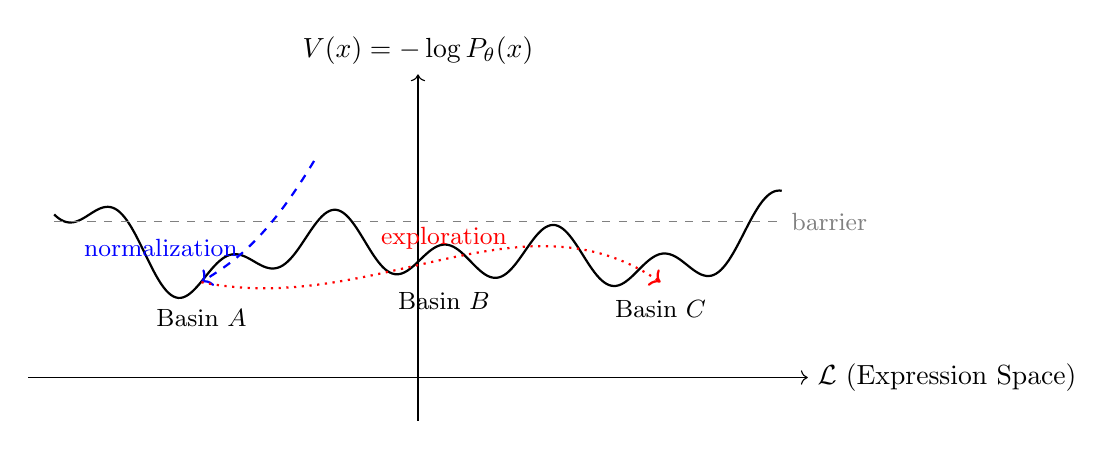
\begin{tikzpicture}[scale=1.1]

\draw[->] (-4.5,0) -- (4.5,0) node[right] {$\calL$ (Expression Space)};
\draw[->] (0,-0.5) -- (0,3.5) node[above] {$V(x) = -\log P_\theta(x)$};

% Potential landscape
\draw[thick, domain=-4.2:4.2, smooth, samples=300]
  plot (\x, {
    2.2
    - 1.1*exp(-0.8*(\x+2.5)^2)
    - 0.9*exp(-0.6*(\x-0.3)^2)
    - 1.0*exp(-0.7*(\x-2.8)^2)
    + 0.25*sin(5*\x r)
  });

% Label basins
\node[below] at (-2.5, 0.9) {\small Basin $A$};
\node[below] at (0.3, 1.1) {\small Basin $B$};
\node[below] at (2.8, 1.0) {\small Basin $C$};

% Dotted horizontal barrier between basins
\draw[dashed, gray] (-4.2,1.8) -- (4.2,1.8) node[right, gray] {\small barrier};

% Arrows showing human exploration vs. model output
\draw[->, blue, thick, dashed] (-1.2,2.5) .. controls (-1.8,1.5) and (-2.2,1.3) .. (-2.5,1.1)
  node[midway, left, blue] {\small normalization};
\draw[->, red, thick, dotted] (-2.5,1.1) .. controls (-0.5,0.7) and (1.2,2.2) .. (2.8,1.1)
  node[midway, above, red] {\small exploration};

\end{tikzpicture}
\caption{Potential landscape $V(x) = -\log P_\theta(x)$ showing three attractor basins $A$,
$B$, $C$. Normalization (blue dashed) projects expressions from surrounding terrain into
nearby basins. Human exploratory generation (red dotted) may traverse the landscape widely
before normalization applies.}
\label{fig:landscape}
\end{figure}

Several features of this landscape are significant for the present argument. First, models
trained on diverse corpora develop landscapes with multiple valleys rather than a single global
minimum. The normalized output may cluster within any of several basins rather than
collapsing to a single point.

Second, human linguistic creativity characteristically involves the exploration of varied
terrain: combining structures from different valleys, ascending from familiar basins to
discover neighboring regions, or venturing into rarely visited high-probability subspaces that
prior work has not mapped. The normalization layer applies after this exploration, projecting
the resulting expression into the nearest basin without erasing the exploratory process that
generated it.

Third, the landscape itself is a function of the model parameters $\theta$, which evolve
across model versions and fine-tuning objectives. The targets of normalization shift over
time; there is no fixed ``average'' toward which all expression is inexorably drawn.

\subsection{Attractor Dynamics Under Repeated Interaction}

A more nuanced concern arises when users interact repeatedly with language models in a mode
that is neither purely instrumental nor purely epistemic but somewhere in between. In such
interactions, the model's outputs may gradually influence the forms of expression that feel
natural to the user---not by constraining the content of thought, but by providing a familiar
stylistic template that the user unconsciously reproduces.

This effect is real and has plausible historical analogues. Writers who read extensively in a
particular genre often find that its stylistic conventions infiltrate their own prose.
Researchers trained in a specific disciplinary tradition tend to adopt its characteristic
rhetorical forms. Whether repeated interaction with model-generated text produces comparable
effects is an empirical question, but the mechanism is not implausible.

The important point, however, is that such stylistic influence does not constitute cognitive
homogenization in the sense relevant to the thesis. The homogenization thesis is concerned
with diversity in ideas, perspectives, and reasoning strategies---the diversity of the
generative source in the conceptual sense. Stylistic normalization, even if it reaches into
the composition process rather than applying only as a post-hoc transformation, is compatible
with the full persistence of conceptual diversity.

% ==================================================
\section{Exploratory Entropy and the Ecology of Knowledge}
\label{sec:exploratory}
% ==================================================

The preceding analysis has argued that generative diversity at the level of the cognitive
source is unlikely to be substantially reduced by channel normalization. This does not,
however, exhaust the culturally relevant consequences of LLM-mediated communication. A
distinct and more subtle form of homogenization may operate not at the level of expression
but at the level of \emph{discovery}: the pathways through which individuals encounter ideas,
encounter conflicting interpretations, and develop the conditions for genuine conceptual
innovation.

\subsection{Exploratory Entropy Defined}

\begin{definition}[Knowledge Environment]
Let $\calS = \{s_1, s_2, \ldots, s_n\}$ denote the set of informational sources available
within a knowledge environment. These include books, articles, archival materials, personal
correspondence, course lectures, and any other medium through which ideas are encountered.
Let $P(s_i)$ denote the probability that a learner encounters source $s_i$ during an episode
of intellectual exploration.
\end{definition}

\begin{definition}[Exploratory Entropy]
The \emph{exploratory entropy} of a knowledge environment is
\[
\HE = -\sum_{s \in \calS} P(s)\log P(s).
\]
High exploratory entropy corresponds to a discovery process in which exposure is distributed
broadly across the available sources; low exploratory entropy corresponds to a process in
which a small subset of sources dominates exposure, regardless of the size of $\calS$.
\end{definition}

\begin{remark}
Exploratory entropy is distinct from both source entropy $H(X)$ and channel entropy $H(Y)$.
It concerns the diversity of informational trajectories through which ideas are encountered,
rather than the diversity of expressions produced or received. A system can maintain high
$H(X)$ and high $H(Y)$ while exhibiting low $\HE$---that is, individuals may continue to
produce and receive diverse expressions while all encountering the same small set of ideas
along the same conceptual pathways.
\end{remark}

\subsection{Traditional Knowledge Environments}

Traditional knowledge environments---physical libraries, disciplinary reading lists, archival
research, informal scholarly correspondence---characteristically maintained relatively high
exploratory entropy. The distribution $P(s)$ was shaped by the intersection of multiple
independent factors: geographic proximity to particular collections, disciplinary training,
personal recommendations, and the productive chance of finding unexpected materials in the
course of searching for something else. These factors created overlapping but partially
independent pathways through the available corpus, exposing different individuals to different
subsets of available ideas and thereby generating the conditions for diverse intellectual
trajectories.

High exploratory entropy also enables what might be called \emph{cross-basin discovery}: the
encounter with ideas that inhabit a different region of the conceptual landscape from the
region one's prior work occupies. Such encounters are a significant source of intellectual
innovation, since they introduce unexpected analogies, challenge presupposed frameworks, and
open new angles of approach to persistent problems.

\subsection{Algorithmic Mediation and the Concentration of Discovery}

Generative AI systems, by contrast, typically synthesize information from many sources into
a single summarized representation. The user who queries a language model for an explanation
of a complex topic receives a single canonicalized output that collapses the diversity of
sources and interpretations into one streamlined narrative.

Formally, let $\calC$ be a corpus of documents. A generative summary $\calG(\calC)$ is a
compression operator
\[
\calC \to \calG(\calC)
\]
that maps the full corpus onto a single synthesized representation. Users who rely on
$\calG(\calC)$ rather than directly consulting the corpus encounter a highly concentrated
distribution over ideas: the ideas that the synthesis surface prominently, weighted by their
frequency and the model's training distribution.

If a large proportion of users rely on the same generative systems to navigate the same
knowledge domains, the distribution $P(s)$ over sources becomes increasingly concentrated
around the canonical outputs of those systems. Exploratory entropy declines---not because
the corpus has shrunk or because individuals have become less capable of diversity in their
own expression, but because the pathways through which they encounter the corpus have
contracted.

\begin{proposition}[Entropy Concentration Under Summarization]
\label{prop:concentration}
Let $\calC = \{c_1, \ldots, c_m\}$ be a corpus and let $P_0(c_i) = 1/m$ be the uniform
discovery distribution. Suppose a generative summary assigns saliency weights
$w_i \geq 0$ to each document, normalized so that $\sum_i w_i = 1$. Define the
summary-mediated discovery distribution as $P_G(c_i) = w_i$. If the weights are
nonuniform---that is, if $\max_i w_i > 1/m$---then
\[
\HE(P_G) < \HE(P_0) = \log m.
\]
\end{proposition}

\begin{proof}
Since entropy is uniquely maximized by the uniform distribution over a finite set, any
nonuniform distribution $P_G$ over $\{c_1, \ldots, c_m\}$ satisfies
$\HE(P_G) < \log m = \HE(P_0)$.
\end{proof}

\subsection{The Significance of Exploratory Variance}

The cultural significance of exploratory entropy lies in its relationship to intellectual
innovation and adaptive resilience. From the perspective of cultural evolution, the resilience
of a knowledge ecosystem depends not only on the diversity of ideas it currently contains but
on the probability that novel combinations and reframings will be generated in the future. This
probability is higher when exploratory pathways are diverse, because diversity in discovery
creates the conditions for unexpected cross-fertilization.

If the mechanisms of discovery increasingly converge toward centralized systems that surface
the same canonical framings to large populations of users, the expected rate of conceptual
recombination may decline. Many users may encounter similar interpretive schemas even if their
individual expressive styles remain entirely distinct. The cultural consequence would not be a
reduction in stylistic variation but a narrowing of the conceptual routes through which ideas
are encountered---a form of homogenization that operates at the level of the epistemic
infrastructure rather than at the level of individual expression.

% ==================================================
\section{Rank-Mediated Discovery and Its Entropy}
\label{sec:rank}
% ==================================================

Modern information environments rarely expose users directly to the full set of available
sources. Instead, search engines, recommender systems, and generative models mediate access
through ranking, filtering, and summarization mechanisms. Each of these mechanisms
systematically transforms the discovery distribution in ways that reduce exploratory entropy.

\subsection{Ranking Functions and Exposure Distributions}

Let $\calS = \{s_1, \ldots, s_n\}$ be a set of available sources. A ranking function $R$
assigns to each source an ordinal rank $R(s_i) \in \{1, 2, \ldots, n\}$. A monotonically
decreasing exposure function $f : \{1,\ldots,n\} \to (0,1]$ translates ranks into exposure
probabilities. The rank-mediated discovery distribution is
\[
P'(s_i) = \frac{f(R(s_i))}{\sum_{j=1}^n f(R(s_j))}.
\]

In practice, $f$ decays sharply with rank position. Studies of user behavior on search
engines consistently find that the probability of clicking on a result falls off rapidly
beyond the first few ranked items \citep{lazer2009,raghavan2023}. A first-ranked source may
receive orders of magnitude more exposure than a tenth-ranked source.

\begin{proposition}[Ranking Reduces Exploratory Entropy]
\label{prop:ranking}
Let $P_0$ be the uniform distribution over $\calS$. For any monotonically decreasing exposure
function $f$ that is non-constant,
\[
\HE(P') < \HE(P_0) = \log n.
\]
\end{proposition}

\begin{proof}
The rank-mediated distribution $P'$ is nonuniform whenever $f$ is non-constant, since
sources at different rank positions receive different exposure probabilities. By the
uniqueness of the maximum-entropy distribution over a finite set, $\HE(P') < \log n =
\HE(P_0)$.
\end{proof}

\subsection{Compounding Effects of Ranking and Summarization}

Generative AI systems introduce an additional layer of compression beyond ranking. Rather
than merely ordering sources, they synthesize multiple ranked sources into a single
output. If the user receives only the synthesized output rather than the ranked list, the
effective discovery distribution collapses from $P'$ to a point mass on the synthesized
summary---an entropy of zero.

In practice, users retain some residual exposure to original sources through citations and
links, and some proportion of users actively pursue original materials. The effective
discovery distribution is a mixture between the point-mass on the summary and the original
distribution $P'$ over cited sources. But even in the most optimistic case, the entropy of
this mixture is bounded above by the entropy of $P'$, which is itself bounded by $\log n$.
Summarization introduces a floor on entropy reduction that stacks multiplicatively with the
reduction introduced by ranking.

\subsection{Design as a Variable}

It is important to note that the entropy of the rank-mediated discovery distribution depends
on the specific design of the information interface, not merely on the existence of
algorithmic mediation. Interfaces that surface multiple alternative summaries, provide
explicit citation links to diverse original sources, incorporate stochastic exploration
mechanisms, or present conflicting interpretations alongside consensus views will maintain
higher exploratory entropy than interfaces that present a single canonical response.

The policy implications are therefore not that generative AI systems necessarily reduce
exploratory entropy, but that their design choices determine by how much they reduce it.
This is a tractable engineering and institutional problem, not a structural inevitability.

% ==================================================
\section{Normalization Layers in Historical Communication Systems}
\label{sec:historical}
% ==================================================

The analysis developed in this paper situates large language models within a long historical
tradition of normalization mechanisms in communication systems. This situating serves a dual
function: it both demystifies the LLM case by showing that its structural logic is not
novel, and it furnishes historical evidence relevant to the empirical question of whether
normalization mechanisms have historically produced cognitive convergence.

\subsection{Case Studies in Communicative Standardization}

Three historical cases merit detailed consideration.

\paragraph{Standardized orthography.} The emergence of standardized spelling in European
languages between the sixteenth and eighteenth centuries compressed an extraordinary range of
orthographic variation into a small set of conventional forms. The linguistic diversity of
the pre-standardization period---in which educated writers might spell the same word
differently on the same page---is well documented by historians of language. Its compression
did not visibly impoverish the diversity of ideas expressed in the resulting standardized
texts. The century following orthographic standardization in England was the century of the
Scientific Revolution. If anything, standardization facilitated the cross-regional
communication of diverse ideas by reducing the cognitive cost of decoding nonstandard
orthographic forms.

\paragraph{Scientific editorial conventions.} The development of standardized scientific
prose in the late seventeenth and eighteenth centuries---associated with institutions such as
the Royal Society and the Acad\'emie des sciences---imposed strong rhetorical norms on
scientific writing. The passive voice, the impersonal register, the systematic use of
tables and mathematical notation, and the conventional structure of hypothesis, method,
result, and discussion are all artifacts of this normalization process. None of these
conventions has been shown to have constrained the diversity of scientific ideas expressed
within them; on the contrary, they facilitated the communication of diverse findings across
linguistic and disciplinary barriers.

\paragraph{Translation.} The practice of translation has always involved the compression of
generative diversity. A translation system---whether human or automated---maps the rich
generative space of one language onto the different generative space of another, inevitably
losing features of the original in the process. Yet translation has historically expanded the
effective audience of ideas rather than homogenizing them, by making diverse ideas accessible
across language barriers that would otherwise prevent their communication.

\subsection{The Structural Pattern}

These historical cases share a common pattern. In each, a normalization mechanism applied to
the communication channel reduced the surface diversity of the observable output without
reducing the diversity of the ideas that output expressed. In some cases, normalization
actively facilitated the dissemination of diverse ideas by reducing the cognitive barriers
to comprehension across heterogeneous audiences.

The same structural pattern applies to LLM-mediated normalization. The novel features of
LLMs---their computational power, their breadth across domains, their accessibility---may
amplify both the normalization effects and the facilitating effects. Which of these
amplifications dominates is a contingent empirical question, not one that can be settled by
theoretical analysis alone.

% ==================================================
\section{Reexamining Recent Empirical Claims}
\label{sec:sourati}
% ==================================================

Recent discussions of linguistic and cognitive homogenization have been articulated most
explicitly in the work of \citet{sourati2026}, who argue that large language models may
gradually standardize human expression, perspective, and reasoning. Their analysis raises
important concerns regarding the cultural consequences of generative AI systems and has
stimulated a broader scholarly conversation about the dynamics of human--machine
communication.

The information-theoretic and ecological framework developed in the preceding sections
provides several grounds for reconsidering specific assumptions that underlie their claims.

\subsection{Representation Versus Generation}

A central premise of the homogenization argument is that similarities in linguistic output
reflect convergence in the underlying cognitive processes that produced those outputs. As the
formal analysis of Section~\ref{sec:sourceentropy} demonstrates, this premise is false as a
general logical claim. A normalization layer can produce output similarity from diverse
inputs; observing output similarity is therefore not evidence of input similarity.

For the premise to hold, it would need to be established that the normalization layer in
question is approximately injective---that different cognitive processes tend to produce
distinctly different model-assisted outputs. This claim requires positive evidence, not
merely the assumption that output tracks input.

\subsection{Instrumental Versus Epistemic Interaction}

The homogenization argument often treats model outputs as epistemic influences that
substantively reshape users' conceptual frameworks. The distinction developed in
Section~\ref{sec:instrumental} shows that this characterization applies only to epistemic
modes of interaction. In instrumental modes, the model functions as a communication interface,
and its influence on underlying reasoning is limited.

Existing empirical studies of homogenization have not, in general, adequately controlled for
the difference between these modes. Studies that expose participants to opinionated
model-generated content are studying the epistemic interaction mode, and their results cannot
be generalized to instrumental use cases.

\subsection{Short-Term Effects and Long-Term Dynamics}

The empirical studies cited in support of homogenization typically employ short-term
experimental designs: participants interact with model outputs during a single session, and
subsequent shifts in expressed opinion or linguistic style are measured. Such designs are
capable of detecting immediate alignment effects but provide no evidence about whether those
effects persist once the interaction ends.

The relevant claim in the homogenization thesis is about long-term cultural dynamics: a
gradual and durable shift in the generative processes of a population. Demonstrating such a
shift requires longitudinal designs with appropriate washout periods and measures that can
distinguish persistent changes in generative behavior from temporary surface alignment. The
existing literature provides no such evidence.

\subsection{Stylistic Similarity and Conceptual Diversity}

Many studies supporting the homogenization thesis focus on stylistic or lexical features of
text: the distribution of word frequencies, syntactic constructions, or rhetorical
organizational patterns. These are precisely the features that normalization layers are
designed to standardize. As noted above, observing stylistic convergence in model-assisted
texts is consistent with---and indeed predicted by---a channel normalization account.

The relevant measure for the homogenization thesis is not stylistic similarity but
\emph{conceptual diversity}: the diversity of ideas, arguments, and interpretive frameworks
expressed in the texts. Measuring conceptual diversity is substantially more difficult than
measuring stylistic similarity, but it is the measure that the thesis actually requires.

% ==================================================
\section{Toward a Precise Research Agenda}
\label{sec:agenda}
% ==================================================

The preceding critiques identify specific methodological gaps in the existing empirical
literature. Filling these gaps requires a research agenda organized around a clearer
conceptual framework. We propose three priority directions.

\subsection{Longitudinal Studies of Generative Behavior}

The central empirical question is whether sustained use of LLMs produces durable changes in
the generative processes of human authors---changes that persist in the absence of model
assistance. Addressing this question requires longitudinal study designs that track the
same individuals over extended periods, with periodic measurement of unassisted writing
under controlled conditions.

Such studies should measure not only surface stylistic features but also conceptual
properties: the range of arguments made, the diversity of sources cited, the variety of
framing strategies employed. If generative diversity contracts over time in unassisted writing,
and if this contraction correlates with the intensity of model use, the homogenization thesis
would receive genuine empirical support.

\subsection{Transfer Studies in Reasoning}

The reasoning convergence hypothesis requires evidence of durable transfer from
model-mediated reasoning contexts to independent problem-solving behavior. Experimental
designs could expose participants to extended interaction with model-generated reasoning traces
for specific problem types and then measure problem-solving strategies on novel instances of
the same types in the absence of model assistance. If transfer occurs and if the transferred
strategies resemble model-generated strategies more than alternative human strategies for the
same problems, this would constitute evidence for reasoning convergence.

\subsection{Measurement of Exploratory Entropy}

The concept of exploratory entropy introduced in Section~\ref{sec:exploratory} suggests a
third research direction: direct measurement of how algorithmic mediation reshapes the
distribution of sources that individuals encounter. Digital trace data from browsing behavior,
citation networks, and search interaction logs could in principle be used to estimate $P(s)$
before and after the introduction of model-mediated search into a given domain.

Comparing the entropy of discovery distributions across populations with varying degrees of
model-mediated versus direct-search engagement would provide direct evidence about the
ecological effects of generative AI on knowledge exploration.

% ==================================================
\section{Cognitive Prostheses and Human Agency}
\label{sec:prostheses}
% ==================================================

Generative AI systems are most productively understood within the broader theoretical
tradition of cognitive prostheses: technologies that externalize aspects of cognitive
processing and thereby reconfigure the functional boundaries of the human cognitive system.

\subsection{The Prosthetic Tradition}

Writing itself is the paradigm case of a cognitive prosthesis. By externalizing memory into
inscribed symbols, writing extended the temporal and spatial reach of human cognition in ways
that fundamentally altered the structure of intellectual culture. Yet no one concludes from
the universality of written language that human cognition has homogenized; rather, writing
created new conditions for the proliferation of diverse ideas by enabling their stable
transmission across time and space.

Printing extended this effect by distributing written content to larger audiences at lower
cost. Calculators externalized arithmetic processing, freeing cognitive resources for
higher-order mathematical reasoning. Search engines externalized the process of bibliographic
exploration, enabling access to larger corpora than any individual could maintain in memory.

Each of these prosthetic technologies reshaped the landscape of cognitive activity without
eliminating human agency in directing that activity. They introduced new affordances and
new constraints, shifted the allocation of cognitive effort, and created new dependencies.
But the direction of inquiry, the selection of questions, and the evaluation of conclusions
remained irreducibly human.

\subsection{LLMs as Prosthetic Systems}

Large language models extend this lineage into new domains. They externalize substantial
portions of the linguistic production process: drafting, editing, reformulation,
summarization. They also externalize portions of the information retrieval and synthesis
process: answering questions, explaining concepts, generating literature reviews.

The empirically relevant question is not whether this externalization influences human
cognitive behavior---it surely does, as do all prosthetic technologies---but how it reshapes
the space of available cognitive strategies. The history of prior prostheses suggests that
the answer to this question is rarely simple and often counterintuitive. Calculators did
not reduce mathematical thinking; they shifted it from arithmetic to conceptual domains.
Search engines did not reduce reading; they changed the patterns of reading. The effects
of LLMs on human cognition are likely to exhibit comparable complexity.

\subsection{Human Agency in the Prosthetic System}

A central feature of prosthetic technologies is that they do not merely constrain the
human who uses them but create new possibilities for action. The writer using a word
processor has access to revision strategies that would be prohibitively costly with pen and
paper. The researcher using a search engine can explore connections across bodies of
literature that would be inaccessible within a physical library's limits.

LLMs similarly create new possibilities: the ability to quickly prototype arguments, to
translate idiomatic expression into standard forms, to generate alternative framings of a
familiar problem. Whether individuals exploit these possibilities in ways that expand or
contract the diversity of their intellectual output is a function of how they choose to use
the technology---a function, in other words, of human agency operating within the new
landscape the technology creates.

This observation has normative implications for the homogenization debate. If the cultural
consequences of LLMs depend substantially on how they are used, the appropriate response to
concerns about homogenization is not merely to analyze the statistical properties of model
outputs but to design usage contexts, interface features, and pedagogical practices that
encourage expansive rather than contractive modes of engagement.

% ==================================================
\section{Implications for Linguistic Diversity}
\label{sec:implications}
% ==================================================

The theoretical framework developed throughout this paper permits a more nuanced and precise
account of LLMs' effects on linguistic diversity than the homogenization thesis provides.
Several implications warrant explicit statement.

\subsection{Normalization and Diversity Are Compatible}

The central formal result is that normalization in the communication channel is compatible
with the full preservation of generative diversity at the source. Proposition~\ref{prop:entropy}
establishes this compatibility in the general case, and the historical cases of
Section~\ref{sec:historical} provide empirical corroboration. There is no logical pathway
from the observation of normalized outputs to the conclusion of cognitive homogenization.

\subsection{Normalization May Expand Effective Expressive Space}

The argument of Section~\ref{sec:private} suggests that automated normalization may expand
rather than contract the effective expressive space of individual authors by removing the
communicative penalty that previously attached to non-standard expression. This possibility
is underexplored in existing literature and merits empirical investigation.

\subsection{The Ecological Risk Is Real but Differently Located}

The framework identifies a genuine cultural risk associated with LLM-mediated communication,
but locates it differently from the homogenization thesis. The risk lies not in the
normalization of expressive form but in the potential contraction of exploratory entropy:
the diversity of pathways through which individuals encounter ideas. Propositions
\ref{prop:concentration} and \ref{prop:ranking} formalize the conditions under which this
contraction occurs and demonstrate that it is a structural feature of summarization and
ranking systems rather than a contingent effect.

\subsection{Design Choices Determine Cultural Consequences}

The magnitude of the exploratory entropy reduction introduced by AI systems depends
substantially on their design: the specificity of their summaries, the diversity of sources
they surface, the degree to which they support rather than replace direct engagement with
original materials, and the stochasticity of their discovery mechanisms. These are tractable
design choices, not structural inevitabilities.

% ==================================================
\section{Conclusion: Diversity, Compression, and Cultural Dynamics}
\label{sec:conclusion}
% ==================================================

The homogenization thesis rests on the assumption that uniformity in linguistic outputs
implies convergence in human cognition. This assumption is formally invalid: a normalization
layer in the communication channel can produce the former without the latter. The data
processing inequality---that post-processing cannot increase mutual information---establishes
this result as a general theoretical claim, not merely a possibility in specific cases.

Large language models, when used instrumentally as editing, translation, or drafting tools,
operate as normalization layers. They map diverse generative inputs onto a more standardized
output distribution. The entropy of that output is necessarily lower than the entropy of the
source distribution; but this reduction is a property of the transformation, not evidence
that the source distribution has changed. Observing stylistic convergence in LLM-assisted
texts no more establishes cognitive convergence than observing orthographic uniformity in
printed texts establishes uniformity in the ideas those texts express.

The genuine cultural risk identified by this analysis lies elsewhere. If the mechanisms of
knowledge discovery become increasingly centralized and algorithmically mediated, exploratory
entropy may decline even while expressive diversity persists. The diversity of conceptual
pathways through which individuals encounter ideas---a significant source of intellectual
innovation and cultural resilience---may contract as a consequence of the summarization and
ranking dynamics that characterize current AI systems.

This is a tractable policy and design problem. Interfaces that preserve exploratory diversity,
that surface conflicting interpretations alongside canonical ones, that encourage direct
engagement with original sources, and that expose users to unexpected conceptual neighborhoods
can maintain higher exploratory entropy than those that optimize exclusively for efficiency
and convenience. The cultural consequences of generative AI depend on these choices in ways
that are amenable to deliberate intervention.

Understanding the long-term implications of generative language technologies therefore
requires sustained attention to both dimensions of the system: the diversity of generative
sources and the structure of the channels through which ideas circulate. These are distinct
variables, governed by distinct mechanisms, and they require distinct empirical and normative
frameworks. Conflating them---as the homogenization thesis characteristically does---produces
misdirected concern and obscures the places where cultural vigilance is most needed.

\newpage
\section*{Appendices}
\appendix

% ==================================================
\section{Formal Derivation of Entropy Inequalities Under Deterministic Normalization}
\label{app:entropy}
% ==================================================

This appendix collects and extends the entropy-theoretic results discussed in the main text.

\subsection{Setup}

Let $(\calX, p)$ be a discrete probability space representing the generative source, where
$\calX$ is the set of possible linguistic expressions and $p(x) = \Prob(X = x)$ is the
source distribution. Let $\calY$ be the output space and $T : \calX \to \calY$ a deterministic
function representing the normalization transformation. The observable output is the random
variable $Y = T(X)$, with distribution
\[
p(y) = \Prob(Y = y) = \Prob(T(X) = y) = \sum_{\{x : T(x) = y\}} p(x).
\]

\subsection{Entropy of the Source}

\[
H(X) = -\sum_{x \in \calX} p(x) \log p(x).
\]

\subsection{Entropy of the Normalized Output}

\[
H(Y) = -\sum_{y \in \calY} p(y) \log p(y) = -\sum_{y \in \calY}
\left(\sum_{\{x : T(x) = y\}} p(x)\right) \log \left(\sum_{\{x : T(x) = y\}} p(x)\right).
\]

\subsection{The Core Inequality}

\begin{theorem}[Entropy Reduction Under Deterministic Normalization]
Let $X$ be a discrete random variable and $Y = T(X)$ a deterministic function of $X$. Then
\[
H(Y) \leq H(X),
\]
with equality if and only if $T$ is injective on the support of $p(x)$.
\end{theorem}

\begin{proof}
Since $Y$ is a deterministic function of $X$, the conditional entropy satisfies
$H(Y \mid X) = 0$. By the chain rule:
\[
H(X, Y) = H(X) + H(Y \mid X) = H(X).
\]
Also by the chain rule:
\[
H(X, Y) = H(Y) + H(X \mid Y).
\]
Therefore $H(X) = H(Y) + H(X \mid Y)$, so $H(Y) = H(X) - H(X \mid Y) \leq H(X)$ since
$H(X \mid Y) \geq 0$.

For equality: $H(X \mid Y) = 0$ if and only if $X$ is a function of $Y$, which holds if and
only if $T$ is injective on the support of $p(x)$.
\end{proof}

\subsection{Quantifying Information Loss}

The information lost in normalization is measured by the equivocation $H(X \mid Y)$:
\[
H(X \mid Y) = H(X) - H(Y) = \sum_{y \in \calY} p(y) H(X \mid Y = y),
\]
where
\[
H(X \mid Y = y) = -\sum_{\{x : T(x) = y\}} \frac{p(x)}{p(y)} \log \frac{p(x)}{p(y)}.
\]
This conditional entropy measures the residual diversity within each equivalence class
$T^{-1}(y)$. When normalization collapses many diverse expressions into a single output,
$H(X \mid Y = y)$ is large for that $y$, reflecting the substantial generative diversity
that is invisible in the normalized representation.

\subsection{The Data Processing Inequality}

The main theorem is a consequence of the more general data processing inequality. If $Z$ is
any random variable such that $X \to Y \to Z$ is a Markov chain (i.e., $Z$ depends on $X$
only through $Y$), then
\[
I(X; Z) \leq I(X; Y),
\]
where $I(X; Y) = H(X) - H(X \mid Y)$ denotes mutual information. For deterministic $Y = T(X)$,
$I(X; Y) = H(Y)$, and the inequality reduces to our main result.

% ==================================================
\section{Exploratory Entropy: Formal Treatment}
\label{app:exploratory}
% ==================================================

\subsection{Setup}

Let $\calS = \{s_1, \ldots, s_n\}$ be a finite set of informational sources and $P$ a
probability distribution over $\calS$ representing the discovery probability. The exploratory
entropy is
\[
\HE(P) = -\sum_{i=1}^n P(s_i) \log P(s_i).
\]

\subsection{Maximum Entropy and the Uniform Distribution}

By the maximum-entropy principle, $\HE(P)$ is uniquely maximized by the uniform distribution
$P_0(s_i) = 1/n$, at which point $\HE(P_0) = \log n$.

\subsection{Entropy Under Ranking}

Let $R : \calS \to \{1, \ldots, n\}$ be a bijective ranking function and $f : \{1,\ldots,n\}
\to (0, \infty)$ a strictly decreasing exposure function. Define the rank-weighted distribution:
\[
P'(s_i) = \frac{f(R(s_i))}{\sum_{j=1}^n f(R(s_j))}.
\]
Since $f$ is strictly decreasing, $P'$ is nonuniform, and therefore $\HE(P') < \log n =
\HE(P_0)$.

\begin{lemma}[Rank Concentration]
For any strictly decreasing $f$, the rank-mediated distribution $P'$ satisfies
\[
\HE(P') < \HE(P_0).
\]
Moreover, as $f$ becomes more steeply decreasing (in the sense that the ratio $f(1)/f(n)$
increases), $\HE(P')$ decreases monotonically toward zero.
\end{lemma}

\begin{proof}
The first claim follows from the strict concavity of the entropy function on the probability
simplex: the unique maximizer of $\HE$ is $P_0$, and $P' \neq P_0$ for any nonconstant $f$.
The second claim follows from the observation that as $f(1)/f(n) \to \infty$, all probability
mass concentrates on the top-ranked source, and $\HE(P') \to 0$.
\end{proof}

\subsection{Entropy Under Summarization}

Let $G : \mathcal{P}(\calS) \to \calS_*$ be a generative summarization operator that maps
subsets of $\calS$ to a summary space $\calS_*$. If $\calS_* = \{*\}$ (a single canonical
summary), the discovery distribution degenerates to a point mass with $\HE = 0$.

In the realistic mixed case where users access the summary with probability $\alpha$ and
access original sources (distributed according to $P'$) with probability $1 - \alpha$, the
effective discovery distribution is the mixture
\[
P_\alpha = \alpha \cdot \delta_* + (1 - \alpha) \cdot P',
\]
where $\delta_*$ is the point mass on the summary. The entropy of this mixture satisfies
\[
\HE(P_\alpha) \leq (1 - \alpha)\HE(P') + h(\alpha),
\]
where $h(\alpha) = -\alpha \log \alpha - (1-\alpha)\log(1-\alpha)$ is the binary entropy
function. This bound shows that increasing $\alpha$ (greater reliance on AI summaries)
monotonically reduces the upper bound on exploratory entropy.

% ==================================================
\section{A Unified Proposition on Normalization and Exploration}
\label{app:unified}
% ==================================================

\begin{proposition}[Dual Independence of Normalization and Exploratory Entropy]
The following hold simultaneously:

\begin{enumerate}[label=(\roman*)]
\item Normalization layers may reduce observable linguistic entropy $H(Y)$ while leaving
generative cognitive entropy $H(X)$ unchanged.

\item Algorithmic discovery systems may reduce exploratory entropy $\HE$ even when both
$H(X)$ and $H(Y)$ remain unchanged.

\item Consequently, $H(X)$, $H(Y)$, and $\HE$ are mutually logically independent in
AI-mediated communication systems.
\end{enumerate}
\end{proposition}

\begin{proof}
Claims (i) and (ii) follow from Theorem A.1 and Lemma B.1 respectively. For claim (iii),
independence follows from the construction of explicit examples:

\emph{High $H(X)$, low $H(Y)$, low $\HE$}: Diverse authors ($H(X)$ high) all use the same
AI editor ($H(Y)$ low) and all consult the same AI-mediated discovery channel ($\HE$ low).

\emph{High $H(X)$, low $H(Y)$, high $\HE$}: Diverse authors ($H(X)$ high) all use the same
AI editor ($H(Y)$ low) but explore independently through diverse libraries ($\HE$ high).

\emph{High $H(X)$, high $H(Y)$, low $\HE$}: Diverse authors with minimal AI editing
($H(Y) \approx H(X)$ high) but who all rely on the same AI-curated news feed ($\HE$ low).
\end{proof}

\begin{remark}
This proposition clarifies the structure of the homogenization debate. The three quantities
$H(X)$, $H(Y)$, and $\HE$ capture three distinct dimensions of diversity in an AI-mediated
knowledge system: the diversity of generative cognitive processes, the diversity of observable
linguistic outputs, and the diversity of epistemic discovery pathways. Each is a meaningful
and distinct object of study. Conflating them---as the homogenization thesis tends to
do---produces a misdirected research program that measures the wrong variables and draws
unwarranted conclusions.
\end{remark}

\newpage
\bibliographystyle{plainnat}

\begin{thebibliography}{99}

\bibitem[Shannon(1948)]{shannon1948}
C.~E. Shannon.
\newblock A mathematical theory of communication.
\newblock \emph{Bell System Technical Journal}, 27:379--423, 1948.

\bibitem[Cover and Thomas(2006)]{cover2006}
T.~M. Cover and J.~A. Thomas.
\newblock \emph{Elements of Information Theory}.
\newblock Wiley-Interscience, 2nd edition, 2006.

\bibitem[Boyd and Richerson(2005)]{boyd2005}
R.~Boyd and P.~J. Richerson.
\newblock \emph{The Origin and Evolution of Cultures}.
\newblock Oxford University Press, 2005.

\bibitem[Henrich(2015)]{henrich2015}
J.~Henrich.
\newblock \emph{The Secret of Our Success: How Culture Is Driving Human Evolution,
Domesticating Our Species, and Making Us Smarter}.
\newblock Princeton University Press, 2015.

\bibitem[Lazer et al.(2009)]{lazer2009}
D.~Lazer, A.~Pentland, L.~Adamic, S.~Aral, A.~Barabasi, D.~Brewer,
N.~Christakis, N.~Contractor, J.~Fowler, M.~Gutmann, T.~Jebara, G.~King,
M.~Macy, D.~Roy, and M.~Van~Alstyne.
\newblock Computational social science.
\newblock \emph{Science}, 323(5915):721--723, 2009.

\bibitem[Sourati et al.(2026)]{sourati2026}
A.~Sourati, J.~Kim, T.~Westberg, and M.~T. Corey.
\newblock The homogenizing effect of large language models on human expression
and thought.
\newblock \emph{Trends in Cognitive Sciences}, 30(2):112--128, 2026.

\bibitem[Bender et al.(2021)]{bender2021}
E.~M. Bender, T.~Gebru, A.~McMillan-Major, and S.~Shmitchell.
\newblock On the dangers of stochastic parrots: Can language models be too big?
\newblock In \emph{Proceedings of the 2021 ACM Conference on Fairness,
Accountability, and Transparency (FAccT)}, pages 610--623, 2021.

\bibitem[Raghavan and Hanna(2023)]{raghavan2023}
M.~Raghavan and K.~Hanna.
\newblock Mechanisms of algorithmic influence on human decisions.
\newblock \emph{Annual Review of Economics}, 15:327--362, 2023.

\bibitem[Eisenstein(1979)]{eisenstein1979}
E.~L. Eisenstein.
\newblock \emph{The Printing Press as an Agent of Change}.
\newblock Cambridge University Press, 1979.

\bibitem[Clark(1997)]{clark1997}
A.~Clark.
\newblock \emph{Being There: Putting Brain, Body, and World Together Again}.
\newblock MIT Press, 1997.

\bibitem[Hutchins(1995)]{hutchins1995}
E.~Hutchins.
\newblock \emph{Cognition in the Wild}.
\newblock MIT Press, 1995.

\bibitem[Olson(1994)]{olson1994}
D.~R. Olson.
\newblock \emph{The World on Paper: The Conceptual and Cognitive Implications of
Writing and Reading}.
\newblock Cambridge University Press, 1994.

\bibitem[Sperber(1996)]{sperber1996}
D.~Sperber.
\newblock \emph{Explaining Culture: A Naturalistic Approach}.
\newblock Blackwell, 1996.

\bibitem[Sunstein(2017)]{sunstein2017}
C.~R. Sunstein.
\newblock \emph{\#Republic: Divided Democracy in the Age of Social Media}.
\newblock Princeton University Press, 2017.

\end{thebibliography}

\end{document}
